
\section[Branching Strategies]{Branching Strategies}


\subsection[]{Centralized Workflow}
\begin{frame}
\frametitle{Centralized Workflow}
\begin{columns}
          \column{0.5\linewidth}
		\begin{itemize}
		\item Master branch only.
		\item Easier transition to Git.
		\item Users don’t need to change their workflow.
		\end{itemize}
          \column{0.5\linewidth}
		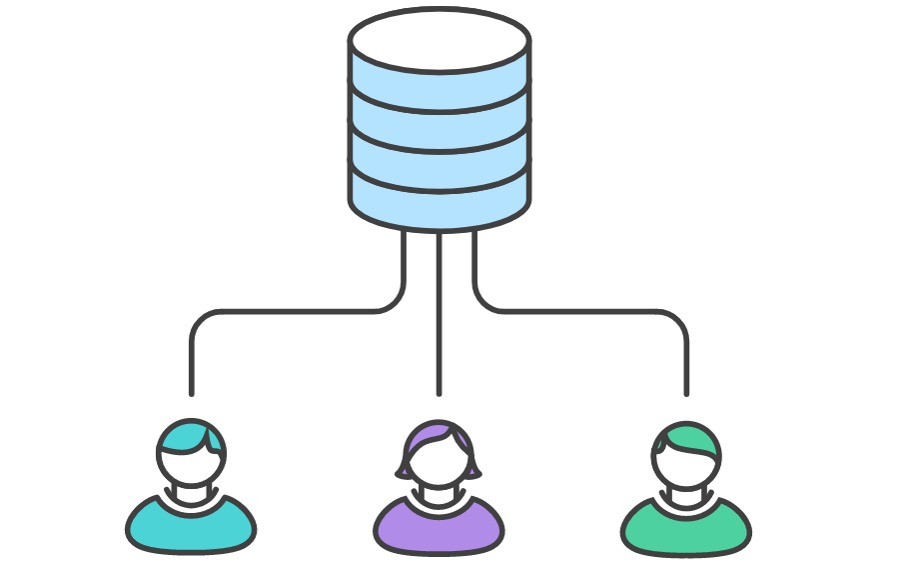
\includegraphics[width=\textwidth, height=0.62\textwidth]{centralized-workflow.png}
\end{columns}
\end{frame}

\subsection[]{Feature Branch Workflow}
\begin{frame}
\frametitle{Feature Branch Workflow}
\begin{itemize}
	\item Feature development isolated in feature branches – pull request for discussing the changes.
	\item Master branch should always hold stable code.
\end{itemize}
\begin{center}
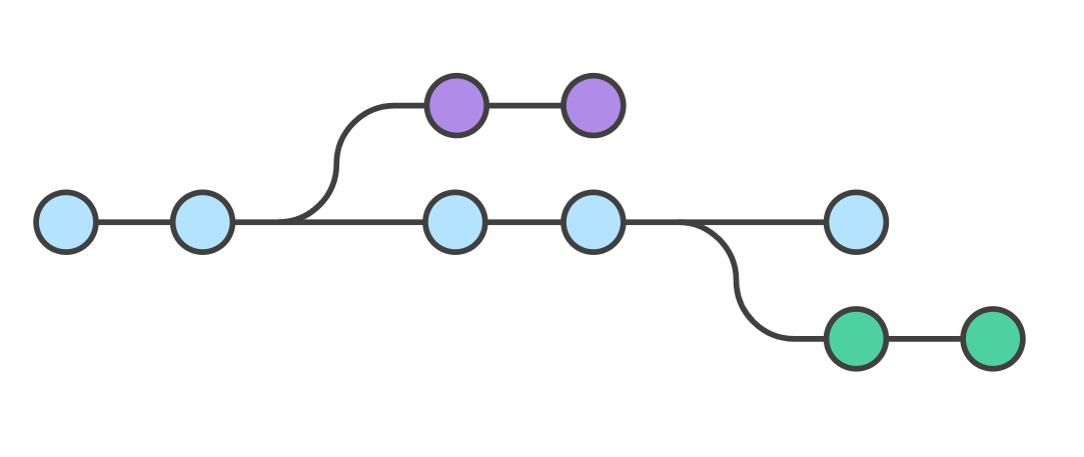
\includegraphics[width=\textwidth, height=0.42\textwidth]{feature-branch-workflow.png}
\end{center}
\end{frame}

\subsection[]{Gitflow Workflow}
\begin{frame}
\frametitle{Gitflow Workflow}
\begin{itemize}
	\item Strict branching model designed around the project release.
		\begin{itemize}
		\item The master branch stores the official release history.
		\item The develop branch serves as an integration branch for features.
		\end{itemize}
\end{itemize}
\begin{center}
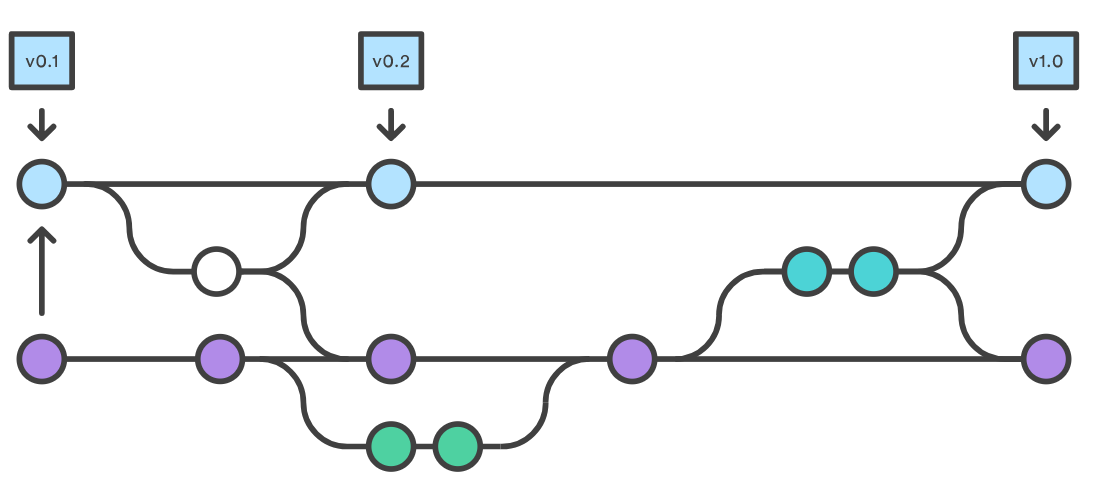
\includegraphics[width=\textwidth, height=0.44\textwidth]{gitflow-workflow.png}
\end{center}
\end{frame}

\subsection[]{Forking Workflow}
\begin{frame}
\frametitle{Forking Workflow}
\begin{columns}
          \column{0.5\linewidth}
		\begin{itemize}
		\item Forks of the repository need to be created.
		\item Each user has a personal public repository.
		\item Project maintainer integrates the changes into official repository via pull requests.
		\item official repository = public repository of project maintainer.
		\end{itemize}
          \column{0.5\linewidth}
		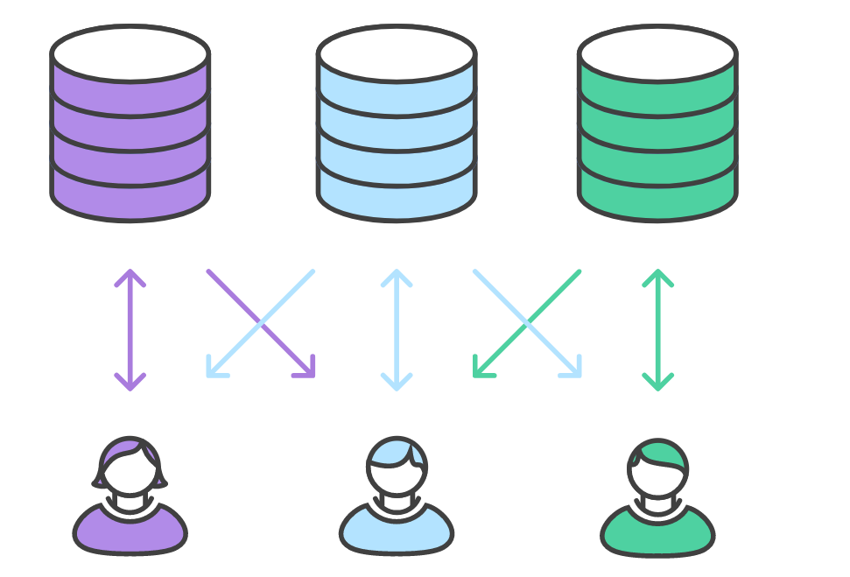
\includegraphics[width=\textwidth, height=0.68\textwidth]{forking-workflow.png}
\end{columns}
\end{frame}

\subsection[]{Tools Overview}
\begin{frame}
\frametitle{Tools Overview}
\begin{itemize}
	\item GitHub, Bitbucket, GitLab etc.
	\item Feature overview:
		\begin{itemize}
		\item Git repository management.
		\item Access control.
		\item Branch permissions.
		\item Pull requests with code reviews and comments.
		\item Code aware search.
		\item Git Large File Storage (LFS).
		\item 3rd party integrations (Jira, CI server etc.)
		\end{itemize}
\end{itemize}
\end{frame}
